
\section{Permutation}
\subsection{Introduction}

Permutation is a fundamental concept in cryptography. It is used in various cryptographic algorithms such as block ciphers, hash functions, and stream ciphers. A permutation is a bijective mapping from a set to itself. While it is a simple operation, it is actually one of the most important concepts used within the ASCON family. \par


\subsection{Permutation in ASCON}
The ASCON family uses the concept of permutation in its design. The components of the encryption and hashing schemes are the two 320-bit permutations $p^a$ and $p^b$, where $a$ and $b$ are the number of times the round transformations are performed. For example, the parameters for ASCON-128 are $a = 12$ and $b = 6$, while being $a = 12$ and $b = 8$ for ASCON-128a. The permutation function is based on a substitution-permutation network (SPN) structure. \cite{DBLP:journals/joc/DobraunigEMS21, ascon_specification} \par

\subsubsection{Substitution-Permutation network}

It is a type of block cipher that uses a series of substitution and permutation operations.


\begin{center}
  \centering 
  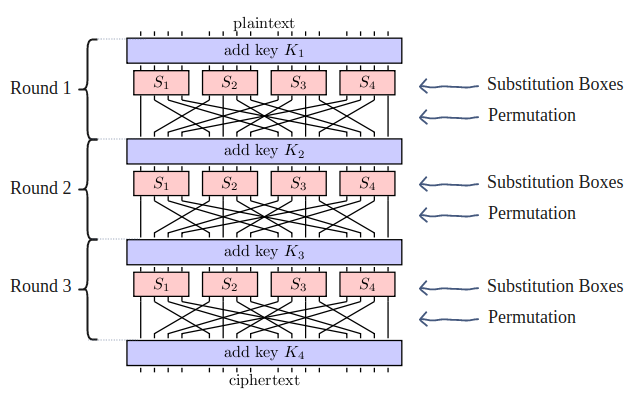
\includegraphics[width=0.6\textwidth]{images/spn.png}
  \captionof{figure}{SPN structure. \cite{DBLP:journals/joc/DobraunigEMS21}}
  \label{fig:spn}
\end{center}

SPN structures consists of boxes called S-boxes that perform substitution operations and P-boxes that perform permutation operations. The S-boxes and P-boxes transform (sub-)blocks of input bits into output bits. Some common operations include simple and efficient XOR and bitwise rotation. \cite{mustafeez}

In the case of ASCON, the round transformation $p$ is based on an SPN structure. It consists of three main components: the constant addition  layer $p_C$, the substitution layer $p_S$, and the linear diffusion layer $p_L$. \cite{DBLP:journals/joc/DobraunigEMS21, ascon_specification} \par

\[p=p_C \circ p_S \circ p_L\]

In order to prepare the 320-bit state for the round transformations, the state is first divided into five 64-bit words. The round transformation $p$ is then applied to the state. \cite{DBLP:journals/joc/DobraunigEMS21} \par 

\begin{center}
  \centering 
  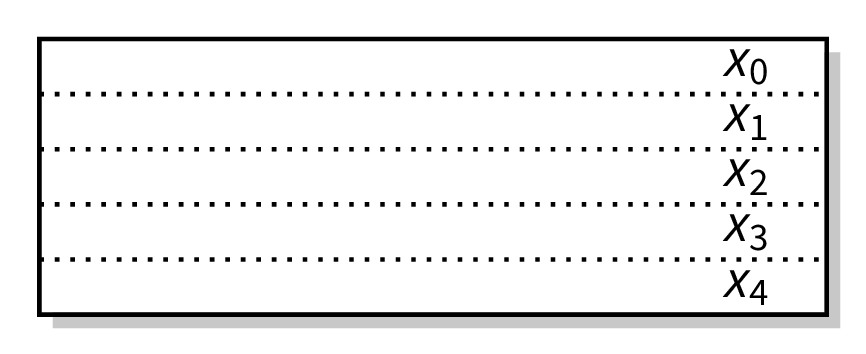
\includegraphics[width=0.5\textwidth]{images/state.png}
  \captionof{figure}{The state divided into 5 64-bit words. \cite{ascon_specification}}
  \label{fig:state}
\end{center}

In each round of the permutation $p$ of ASCON, the following operations are performed:

\subsubsection{Constant addition layer $p_C$}
In $p_C$, a round specific 1-byte constant is XORed to $x_2$. \cite{ascon_specification, analysis_of_ascon}

\begin{center}
  \centering 
  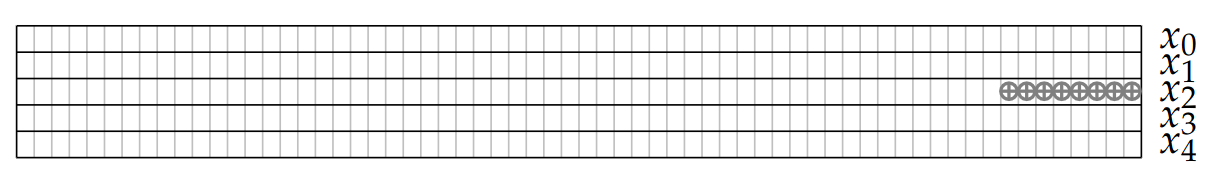
\includegraphics[width=0.8\textwidth]{images/constant.png}
  \captionof{figure}{The constant addition layer $p_C$. \cite{DBLP:journals/joc/DobraunigEMS21}}
  \label{fig:constant}
\end{center}

\subsubsection{Substition layer $p_C$}
In $p_S$, a 5-bit S-box is applied to each byte of the state. It is the application of a 5-bit S-box 64 times in parallel vertically. \cite{ascon_specification, analysis_of_ascon}

\begin{figure}[htbp]
  \centering
  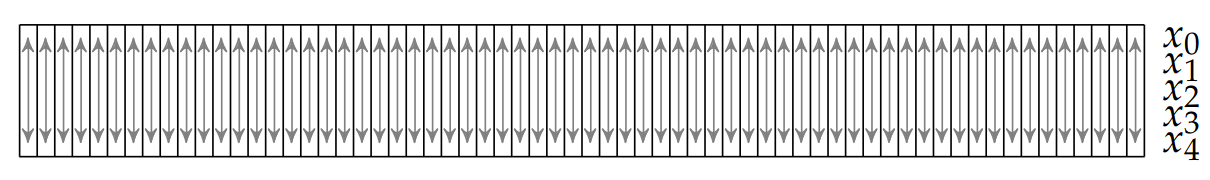
\includegraphics[width=0.8\textwidth]{images/substitution.png}
  \caption{The substitution layer $p_S$.}
  \label{fig:substition}
\end{figure}

\subsubsection{Diffusion layer $p_C$}
in $p_L$, a linear diffusion matrix is applied to the state which only consists of XOR and right rotation of the 64-bit words $x_0, x_1, x_2, x_3, x_4$. \cite{ascon_specification, analysis_of_ascon}

\begin{figure}[htbp]
  \centering
  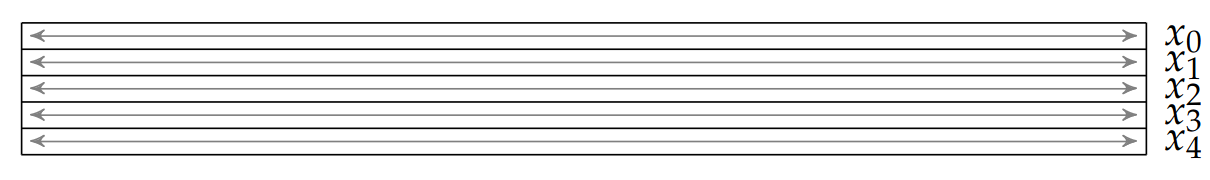
\includegraphics[width=0.8\textwidth]{images/diffusion.png}
  \caption{The diffusion layer $p_L$. \cite{DBLP:journals/joc/DobraunigEMS21}}
  \label{fig:diffusion}
\end{figure}

The linear layer can be described as follows:


$\sum_0 (x_0) = x_0 \oplus (x_0 \ggg 19) \oplus (x_0 \ggg 28)$

$\sum_1 (x_1) = x_1 \oplus (x_1 \ggg 61) \oplus (x_1 \ggg 39)$

$\sum_2 (x_2) = x_2 \oplus (x_2 \ggg 1) \oplus (x_2 \ggg 6)$

$\sum_3 (x_3) = x_3 \oplus (x_3 \ggg 10) \oplus (x_3 \ggg 17)$

$\sum_4 (x_4) = x_4 \oplus (x_4 \ggg 7) \oplus (x_4 \ggg 41)$ 

\cite{ascon_specification,analysis_of_ascon}


\subsection{Design of the permutation}

There are several design criteria that need to be considered when designing a permutation for cryptographic purposes. In ASCON, security was prioritised, but performance was also taken into account. \par

For the constant addition layer $p_C$, the round constants are chosen to prevent certain types of attacks and are added to the state in a simple, predictable manner for ease of computation. They are positioned strategically to facilitate efficient pipelining with other operations. \par

The S-box used in the substitution layer $p_S$ is carefully designed to meet various criteria, including invertibility, resistance against differential and linear cryptanalysis, and efficient implementation in hardware and software. \par

The linear diffusion layer mixes the bits within each word of the state. It is designed to resist linear and differential cryptanalysis while providing good diffusion. The rotation constants are chosen similar to those used in SHA-2 functions to balance performance and security. \cite{DBLP:journals/joc/DobraunigEMS21} \par




